\renewcommand{\chaptername}{Chapter} 
\chapter{Computational foundations: The reverse-correlation method}\label{chap3}

\jj{revoir l'organisation hiérarchique des sections (ex. classification image comme sous partie de revcor)\\ intégrer palin et illustrer avec des simulations}

\section {Psychophysics} 
The mind and body, though different in nature, are not separate entities under the viewpoint of Double aspectism. This was the belief of Gustave Fechner, who sought to uncover the relationship between neurons, synapses, and the processes that give rise to thought, emotions, consciousness, and more. Fechner strongly believed in the power of empirical evidence, emphasizing the importance of observation and experimentation, that was the start of experimental psychology. His ambition was to find a way to measure the mind. In 1860, he laid the foundation for psychophysics, a science dedicated to understanding the relationship between the physical and mental worlds. Psychophysics not only investigates how our senses operate but also explores how the mind interprets sensory information.

Psychophysics is essential because the precise measurement of perception provides a foundation for developing theories about how mental representations are formed and processed, it has not only advanced theoretical understanding but has also made powerful predictions about neural mechanisms that were later confirmed by physiological studies. 

Quantitative measurements started very first in the 1830s with Fechner conducting detection tasks for the presence or absence of a stimulus, using the concept of the absolute threshold, which defined the minimum intensity of a stimulus detectable 50\% of the time  based on the decision criterion of one. This was complemented by Ernst Weber’s introduction of discrimination tasks, particularly the difference threshold and the just-noticeable difference (JND) in 1834. These tasks, often conducted using formats as 2AFC (Two-Alternative Forced Choice) presented two options for the participant to choose the one containing the target stimulus or 2IFC (Two-Interval Forced Choice) presented stimuli sequentially in two intervals, requiring the participant to identify the interval with the target, quantified the smallest detectable change in a stimulus to find their detection threshold. Weber established that the JND ($\Delta I$) is proportional ($k$) to the stimulus intensity ($I$), a principle known as Weber’s Law. \cite{falmagne_elements_1985}
\begin{align}
\frac{\Delta I}{I}& = k 
\end{align}

In 1860, Fechner extended this work with Fechner’s Law \cite{johnson2002}, proposing that perceived intensity ($S$) scales logarithmically with physical stimulus intensity ($I$), linking perception to cumulative JNDs.  These tasks were often performed as scaling tasks, where participants rated the intensity of stimuli, providing insight into how perception compresses physical intensities into manageable representations.
\begin{align}
S& = k \log(I) + C
\end{align}
The results of such experiments are often visualized using a psychometric curve, which plots the probability of a participant’s response (e.g., detection or discrimination) against the physical intensity of the stimulus. This curve, typically S-shaped, allows researchers to estimate thresholds (e.g., the absolute threshold or JND) and analyze how sensitivity changes with stimulus intensity.

Meanwhile, Hermann von Helmholtz advanced sensory physiology with his Trichromatic Theory of Color Vision, which likely involved discrimination tasks to distinguish or match colors using primary lights (red, green, and blue). His Place Theory of Hearing employed 2IFC tasks to assess pitch discrimination, highlighting how different frequencies activate specific regions of the cochlea.  \cite{yost_human_1993}

Later, in 1957, Stevens’ Power Law generalized Fechner’s logarithmic model, showing that perception could follow linear, logarithmic, or exponential relationships depending on the sensory modality. Stevens employed scaling tasks where participants estimated perceived intensities using rating scales or proportional judgments.
\begin{align}
S& = k I^n
\end{align}
These milestones, integrating detection tasks, discrimination tasks, and scaling tasks, formed the foundation of modern psychophysics, advancing our understanding of sensory thresholds, perceptual scaling, and the intricate relationship between physical stimuli and subjective experience.

\section {Signal detection theory} 
The development of Signal Detection Theory (SDT) in 1966 by David M. Green and John A. Swets \cite{d_m_green_and_j_a_swets_signal_1966} marked a significant advance in psychophysics. SDT addressed limitations in earlier methods, which could not effectively estimate false positives (false alarms) or distinguish them from true detections. Traditional threshold-based approaches assumed that detection was solely based on sensory sensitivity, failing to account for the influence of decision-making factors and overcame these issues by distinguishing between perceptual sensitivity ($d'$) and response bias ($\beta$). Unlike traditional threshold-based approaches, SDT introduced a probabilistic framework, emphasizing that detection depends on both the actual sensory signal and the subject's decision-making process. Key tools, like Receiver Operating Characteristic (ROC) curves, allowed researchers to analyze the trade-off between hit rates ($z(H)$) and false alarms ($z(FA)$), separating true sensory ability from contextual factors.  
\begin{align}
d'& = z(H)- z(FA)
\end{align}
\begin{align}
\beta& = -\frac{z(H) + z(FA)}{2}
\end{align}
\section {Decision making} 
Signal Detection Theory (SDT) is based on how we detect a signal from various sensory stimuli amidst noise ($signal+noise$). In the case of neurons that fire in response to stimuli, the detector responsible for processing these signals also generates activity influenced by internal noise, leading to variability. Similarly, in humans performing sensory discrimination tasks, the ability to make decisions based on stimuli is not only influenced by the subjective criterion of the individual but also limited by internal noise. By analyzing the distribution of internal noise and the response criterion, SDT provides a framework to understand how humans encode stimuli and make decisions under uncertainty.

\section {Reverse correlation} 
Building on the foundation of Signal Detection Theory and decision-making frameworks, researchers have approached the brain as a nonparametric system to probe its internal representations . In this context, stimuli are treated as inputs to the system, while the resulting responses represent the system's outputs. This perspective has driven the development of methods like system identification, which aims to uncover the underlying rules and mechanisms that govern how sensory systems process information.

Reverse correlation is widely used to measure the receptive fields of visual neurons by analyzing their responses to random or structured inputs, such as white noise. These approaches have provided critical insights into spatial and color processing in the cortex at low-level processing in early sensory areas as V1. \cite{marmarelis_analysis_1978}

In its neurophysiological origins, random stimuli are presented to a sensory neuron, and cross-correlations between white noise stimuli and sparsely occurring neuronal spikes are computed more efficiently by focusing on segments preceding the spikes. By averaging the stimuli that generated a response, the spike-triggered average (STA) is obtained, representing the weights of a linear filter that approximates the neuron's response and reflects its preferred stimulus under the assumption of linearity which has been called the spatio-temporal impulse response, effectively describing their input-output relationship.

\section {Kernels} 
In Black-box system identification, Volterra and Wiener kernel methods \cite{eggermont_wiener_1993}are powerful tools for understanding complex systems with time-varying inputs $x(t)$ and outputs $y(t)$, such as photoreceptors responding to changes in luminance. Volterra (1930) and Wiener (1958) demonstrated that under certain conditions (e.g., time invariance and finite memory), such systems can be approximated as a sum of simpler subsystems. These include a zero-order subsystem in Volterra kernel, which produces a constant output, a first-order subsystem, which generates a weighted sum of past inputs using the first-order kernel, and a second-order subsystem, which captures pairwise interactions of past inputs through the second-order kernel.
Wiener kernels, an orthogonalized version of Volterra kernels, simplify the estimation process and can be measured using white noise inputs. Lee and Schetzen (1965) showed that white noise, having a flat power spectral density, enables the direct calculation of correlations between input and output to estimate the kernels. For instance, the zero-order kernel corresponds to the average output, the first-order kernel is derived from the correlation between input and output, and the second-order kernel involves correlations between pairs of inputs and the residual output. 


\section {Classification images} 

In visual psychophysics, the first-order kernel (Wiener kernel) is referred to as the classification image experiment. Unlike traditional kernel methods that analyze continuous inputs and outputs distributed over time, this approach presents $signal+noise=stimulus$ (noise field) as discrete pixels in two-dimensional space to human participants. The observer provides a single discrete response, rather than a continuous variable output over time.
In a typical experiment, the stimulus consists of one of two possible signals embedded in a Gaussian noise field that varies from trial to trial. The observer’s task is to identify which signal was shown on each trial.

Ahumada \cite{ahumada_classification_2002} introduced a method for calculating classification images by analyzing the correlation between noise fields and participant responses. The process involves averaging the noise from trials with negative responses and subtracting the average noise from trials with positive responses. The resulting classification image (correlation matrix) visualizes how noise at each point influences the observer's decisions.
\begin{align}
c &= (n_{12} + n_{22}) - (n_{11} + n_{21})
\end{align}
Beyond classification images, the bubbles technique, a variant of reverse correlation, has gained popularity in vision sciences in identifying the features human observers use in detection and discrimination tasks by windowing stimuli across multiple spatial scales (\cite{gosselin_bubbles_2001}\cite{gosselin_superstitious_2003}; Dupuis-Roy et al., 2009 ).

In the auditory domain, random perturbations are applied to signal processing representations, such as spectrograms or speech synthesis models. In this context, the classification image is often referred to as weights, as \cite{ahumada_stimulus_1971} used least-squares regression to relate observers’ rating responses to the stimulus energy at each frequency of an auditory spectrogram. The resulting regression coefficients were interpreted as the weights observers assigned to different frequencies when judging the presence of the signal.

\begin{tcolorbox}[title=Palin Toolbox: Simulate experiment and linear observer,
    colback=white!30!white, colframe=blue!80!white]
The Palin toolbox is a Python-based framework for simulating psychophysical experiments, particularly useful for reverse correlation techniques. 

We create an Observer here, a LinearObserver with a True kernel, internal noise, bias and criteria. Let the observer respond to the DoublePassExperiment or SimpleExperiment.
This generates a list of responses (e.g., 0,1,0,0,0,1,1). 
If the observer has non zero internal noise, responses vary due to stochasticity.

\tcblower

\begin{minted}[fontsize=\tiny]{python}
# Define a DoublePassExperiment with 100 trials + 50 repeated trials
exp = DoublePassExperiment(n_trials = 100, n_repeated = 50, 
                           trial_type = Int2Trial, 
                           n_features = 6, 
                           external_noise_std = 100)

# Create an Observer with a random kernel and internal noise
obs = LinearObserver.with_random_kernel(n_features = exp.n_features,
                                        internal_noise_std = 3, 
                                        criteria = 0)

# Generate responses
responses = obs.respond_to_experiment(exp)

# Convert experiment and responses to a DataFrame for analysis
responses_df = Analyser.to_df(exp, responses)

\end{minted}

\end{tcolorbox}


\begin{figure}[ht!]
    \centering
    \includegraphics[width=19cm]{MainLayout/Images/experiment.jpg}
    \caption{\small An example of simulating double-pass experiment and linear observer with Palin toolbox}
    \label{fig:experiment}
\end{figure}


\section {Linear observer model} 
The linear observer originates from control theory, where it is commonly referred to as a state observer, state estimator, or Luenberger observer. Its primary function is to estimate the internal state of a real system using its inputs and outputs, particularly when direct observation of the internal state is impractical. By analyzing measurable outputs and known inputs, a linear observer reconstructs the system’s internal dynamics, enabling effective control and decision-making.

In psychophysics, the linear observer model adapts this concept to describe how an observer performs a perceptual task, such as in classification image experiments. Here, the observer is assumed to have internal templates representing the signals being presented and makes decisions by comparing the similarity of the stimulus (input) to these templates or in other words the observer's responses are a weighted linear combination of the stimulus features, with added noise representing internal variability.

On each trial, the stimulus($g$) is a combination of a signal ($s_k$) and a noise field ($n$):
\begin{align}
g& =s_k+n 
\end{align}
The observer uses a single internal template ($t$) to make decisions. The decision variable ($d$) is computed as the dot product of the stimulus ($g$) with the template ($t$) and adding internal noise ($z$)
\begin{align}
d& =t^\top n+z 
\end{align}
The observer decides based on whether the decision variable ($d$) crosses a fixed threshold ($a$ which is a bias parameter):

If $d>a$, the observer identifies the signal as $s_1$ otherwise, they identify it as $s_2$.
By averaging noise fields associated with specific stimulus-response categories and combining them, the classification image is estimated. for example:
\begin{itemize}
\item $n_{12}$: noise fields averaged over trials where $s_1$ was presented, but the observer incorrectly responded with $2$.
\item $n_{11}$: noise fields averaged over trials where $s_1$ was presented, but the observer correctly responded with $1$.
\end{itemize}
\begin{align}
c &= (n_{12} + n_{22}) - (n_{11} + n_{21}) \label{eq:weighted_sum}
\end{align}
This standard method is the optimal weighted sum regardless of the variance of the observer’s internal noise.

In Signal Detection Theory (SDT) experiments, where the signal is present in one trial and the other contains only white noise, the use of  \ref{eq:weighted_sum} is appropriate and does not pose any issues.
\begin{align}
c& = \left( n_{\text{hit}} + n_{\text{correct rejection}} \right) - \left( n_{\text{false alarm}} +n_{\text{miss}} \right)
\end{align}

However, in reverse correlation experiments, where all trials are modified by randomly adding Gaussian noise, an alternative equation is required to estimate the classification image or perceptual filter as a correlation map. This can be expressed as:
\begin{align}
c_{\text{corr}} &= \bar{n}^2 - \bar{n}^1 \label{eq:corr_map}
\end{align}
where $c_{\text{corr}}$ represents the average of the noise fields across all trials in which the observer responded $r=2$, subtracted by the average across all trials where the observer responded $r=1$, irrespective of which signal was presented \cite{murray_classification_2011}. This result, known as the classification image, can also be referred to as the prototype\cite{macke_estimating_2010}.


\section {Generalized linear models} 

Generalized Linear Models (GLMs) are a broad class of regression-like models that extend traditional linear regression to accommodate dependent variables with distributions beyond the normal, such as Bernoulli, binomial, or Poisson. The GLM framework models the expected value of a dependent variable as a nonlinear function of a linear combination of predictors through a link function, making it highly flexible and adaptable to a variety of data types.

In this framework, the relationship between predictors and the dependent variable is expressed as:
\begin{align}
g(E[y])& = X \beta
\end{align}
where $g(\cdot)$ is the link function,$E[y]$ is the expected value of the dependent variable,$X$ is the design matrix containing the predictors,$\beta$ is the vector of regression coefficients.
GLMs have found widespread use in modeling behavioral, perceptual, and neural data because of their ability to capture complex relationships between predictors and responses. For example, in neural coding, GLMs are commonly employed to model the perceptual coupling between stimulus features and neural activity. In the case of neural spike data, a Poisson GLM is often used, to model the firing rate of a neuron \cite{pillow_spatio-temporal_2008}.

Signal Detection Theory (SDT), can be formulated as a special case of the GLM.  \cite{decarlo_signal_nodate} demonstrated that SDT concepts map directly onto the GLM framework. For example, the logistic regression model, a specific instance of the GLM, relates the probability of a binary response to stimulus intensity or other predictors.\\In logistic regression, the probability of a "signal present" response is modeled as: 
\begin{align}
\text{Logit}(P)& = \beta_0 + \beta_1 x 
\end{align}
where $P$ represents the probability of a response, 
$\beta_0$ is the intercept, $\beta_1$ and  quantifies the relationship between the stimulus feature $x$ and the observer’s response.
 
GLMs also play a crucial role in estimating classification images,as highlighted by \cite{murray_classification_2011} classification images can be estimated by regressing noise fields against responses using the GLM. The resulting regression coefficients provide a precise estimate of the observer's decision weights.
The GLM’s ability to handle non-Gaussian noise distributions further enhances its versatility in perceptual experiments.

One of the key strengths of GLMs lies in their reliance on maximum likelihood estimation (MLE) for parameter fitting. This robust estimation technique determines the regression coefficients ($\beta$) by maximizing the likelihood of the observed data under the assumed model. The likelihood function is given by:
\begin{align}
L(\beta \mid y, X)& = \prod_{i=1}^{n} f(y_i \mid \mu_i),
\end{align}
The maximum likelihood estimates of $\beta$
are obtained by solving:
\begin{align}
\hat{\beta}& = \arg \max_{\beta} \log L(\beta \mid y, X) 
\end{align}
These estimates enable hypothesis testing and model comparison using statistical tools such as the Akaike Information Criterion (AIC), which evaluates the relative quality of different models.


The Bernoulli GLM is a specific instance of the Generalized Linear Model where the dependent variable $y_t$ represents binary outcomes (e.g., 0 or 1), such as the presence or absence of a neural spike in each time bin. It is often used to model probabilistic events where the outcome follows a Bernoulli distribution.

In the Bernoulli GLM framework, the probability of an event (e.g., a spike) is given by:
\begin{align}
P(y_t = 1 \mid X, \vec{k}) &= f(X \vec{k}),
\end{align}
where:
\begin{itemize}
\item  $X$: The design matrix containing stimulus features or covariates.
\item $\vec{k}$: The weight vector (linear filter) representing the influence of each stimulus feature.
\item $f(\cdot)$: The nonlinear activation function that transforms the linear predictor $X \vec{k}$ into a probability. For logistic regression, $f(\cdot)$ is the logistic (sigmoid) function:
\end{itemize} 
  
\begin{align}
f(x) &= \frac{1}{1 + e^{-x}}.
\end{align}

The model is fitted by maximizing the log-likelihood, which is expressed as:
\begin{align}
L &= Y^T \log f(X \vec{k}) + (1 - Y)^T \log(1 - f(X \vec{k})),
\end{align}
where $Y$ is the vector of binary responses (e.g., spikes or no spikes) over time.

The Bernoulli GLM becomes equivalent to logistic regression when the logistic sigmoid function is used as the nonlinearity. Logistic regression fits this model by estimating $\vec{k}$, the weights of the linear predictor, using maximum likelihood estimation. \cite{pillow_spatio-temporal_2008}

\cite{knoblauch_classification_2008} explored the relationship between GLMs and visual classification images, demonstrating through simulations that GLMs offer a principled and robust framework for estimating observer templates. They found that GLMs are more resistant to noise compared to traditional weighted sum methods. Similarly, \cite{mineault_improved_2009} extended these ideas to analyze complex decision-making tasks by includng non-linear relationship wih sparse priors, enhancing GLM utility for sparse data and showing that GLMs can infer a psychophysical observer’s decision process with fewer trials than previously proposed methods. This enables researchers to explore more sophisticated and informative models of decision-making processes while maintaining statistical tractability.

\begin{tcolorbox}[title=Palin Toolbox: Estimating Kernel,
    colback=white!30!white, colframe=blue!80!white]
In Palin we can process kernel estimation using two distinct methods: Weighted Sum (ClassifcationImages) and GLM (Generalized Linear Model). Both methods normalize the resulting kernel for consistent interpretation.
\tcblower

\begin{minted}[fontsize=\tiny]{python}
# Estimate the kernel with Weighted sum  
ClassificationImage.normalize_kernel
(ClassificationImage.extract_single_kernel(data_df=responses_df, 
feature_id='feature', value_id='value', response_id='response'))

# Estimate the kernel with GLM 
GLMKernel.normalize_kernel
(GLMKernel.extract_single_kernel(data_df=responses_df, 
feature_id='feature', value_id='value', response_id='response'))
\end{minted}

\end{tcolorbox}


\begin{tcolorbox}[title=Palin Toolbox: Kernel estimation error,
    colback=white!30!white, colframe=blue!80!white]
This Python code configures and runs a simulation for kernel extraction. It defines parameters for observers, experiments, and analyzers, and performs the simulation over all possible configurations. Creating 3 Simple experiments (resp. with 150, 500, 1000 trials), of the type 2AFC (Int2Trial), where stimuli are 6-dimensional, randomly sampled with a standard deviation of 100, and aims to look at the error of estimation between 2 methods of kernel extraction.
\tcblower

\begin{minted}[fontsize=\tiny]{python}
# Simulate multiple linear observer to look at the Correlation and confidence interval of estimation

observer_params = {'kernel':['random'],'internal_noise_std':np.arange(0,5.1,0.5), 'criteria':[0]}
experiment_params = {'n_trials': [150,500,1000], 'trial_type': [Int2Trial], 
    'n_features': [6],'external_noise_std': [100]}
analyser_params = {'kernel_extractor': [ClassificationImage,GLMKernel],'distance': ['CORR']}
sim_kernel = Sim(SimpleExperiment, experiment_params,  LinearObserver, observer_params, 
                 KernelDistance, analyser_params)
sim_kernel_df = sim_kernel.run_all(n_runs=10)
\end{minted}
\end{tcolorbox}
\begin{figure}[ht!]
    \centering
    \includegraphics[width=14cm]{MainLayout/Images/kernels.jpg}
    \caption{Main Title for First Image \\ \small Subtitle for the first graphic.}
    \label{fig:kernels}
\end{figure}

\section {Internal noise}
Within the framework of Signal Detection Theory (SDT), internal noise refers to the inherent variability in the responses of sensory neurons and the decision-making process. This variability arises from the stochastic nature of neural activity, which limits the reliability and accuracy of perceptual systems. Interestingly, internal noise is not unique to biological systems—signal degradation due to variability is a well-documented phenomenon in electronic systems, such as amplifiers. However, in sensory neurons, internal noise plays a critical role as a limiting factor in signal transduction, influencing both perception and behavioral performance \cite{faisal_noise_2008}.


This variability in neural responses manifests in psychophysics through the shape of the psychometric function, which transitions gradually in a sigmoid curve rather than sharply between sub-threshold and supra-threshold stimuli \cite{burgess_visual_1988}. The presence of internal noise blurs the boundary between detectable and undetectable stimuli, making sensitivity a probabilistic rather than a deterministic measure.


A decision criterion acts as a threshold to classify responses, defining boundaries between decision categories based on the detector's output. The width of the noise distribution fundamentally limits perceptual performance: greater noise reduces the ability to make accurate decisions.

Internal noise, distinct from external variability, is a critical factor in signal detection. When a signal is embedded in external noise (e.g., added Gaussian noise), an ideal observer uses an internal template to match the signal. In the absence of internal noise, this template closely aligns with the signal, enabling accurate detection. However, internal noise necessitates adjustments—such as clipping or rescaling the template—to maintain functionality. These adjustments illustrate how internal variability constrains the observer’s ability to optimize detection, with higher internal noise limiting both the range and accuracy of the template \cite{neri_optimal_2021}.

The internal-to-external noise ratio provides insight into the relative contributions of sensory variability and environmental factors, indicating whether performance is more influenced by internal processes or external conditions. Understanding this relationship is critical for characterizing perceptual sensitivity and decision-making.

\subsection {Double-pass} 
The double-pass experiment is an experimental paradigm designed to isolate and quantify internal noise, distinguishing it from external noise or task-induced variability. By presenting identical stimuli twice on separate trials and analyzing response consistency, this method attributes any inconsistency to internal noise.

To ensure independence, the two presentations of identical stimuli are separated by many intervening trials. For instance, in a two-alternative forced-choice (2AFC) task, the observer is presented with two stimuli (A and B) and their responses across repeated trials are categorized into four possibilities: AA, AB, BB, BA. These response types quantify decision consistency, with greater inconsistency (e.g., frequent AB or BA responses) indicating higher internal noise \cite{murray_optimal_2002}.

\subsection {Internal noise estimates} 
In this approach, as applied to a 2AFC task, the internal response before the addition of internal noise is assumed to follow a normal distribution for both stimulus conditions: one for the ‘target-absent’ stimulus and another for the ‘target-present’ stimulus, with a mean shift proportional to d' (the observer's sensitivity).

Internal noise is modeled as an added Gaussian noise source with standard deviation $\sigma_z$, which differs for repeated presentations of identical stimuli. This variation represents the internal noise responsible for inconsistencies in the observer's responses. On each trial, the observer selects the stimulus with the highest internal response, meaning that both the signal and noise contribute to the decision-making process.

The internal responses to noise ($r_N$) and signal+noise ($r_{S+N}$) stimuli can be expressed as:
\begin{align}
r_N &\sim \mu_N + N(0, \sigma_N) + N(0, \sigma_z), \\
r_{S+N} &\sim S + \mu_N + N(0, \sigma_N) + N(0, \sigma_z).
\end{align}

Here, $\sigma_N$ is the external noise, $\sigma_z$ is the internal noise, and $S$ represents the signal strength. These responses are normally distributed, with variability arising from both internal and external noise.

To normalize the internal responses with respect to external noise (analogous to calculating z-scores), both equations are transformed by subtracting $\mu_N$ (mean of external noise) and dividing by $\sigma_N$. This yields:
\begin{align}
r'_N &\sim N(0, 1) + N(0, \gamma), \\
r'_{S+N} &\sim d'_{in} + N(0, 1) + N(0, \gamma),
\end{align}
where $\gamma = \frac{\sigma_z}{\sigma_N}$, the internal-to-external noise ratio, and $d'_{in} = \frac{S}{\sigma_N}$, the normalized internal signal strength or input sensitivity \cite{diependaele_how_2012}.

This normalization allows internal noise ($\sigma_z$) and sensitivity ($d'_{in}$) to be expressed in units of external noise, facilitating meaningful comparisons across different experimental conditions and observers.


The method estimates internal noise intensity ($\sigma_z$) by analyzing the relationship between two behavioral metrics:

Percentage of correct responses ($\rho$) =sensitivity  reflects the observer’s ability to discriminate between stimuli, which is influenced by both internal noise and external stimulus properties.


Percentage of agreement  ($\alpha$)= response bias across repeated presentationsquantifies response consistency for identical stimuli, with lower agreement indicating higher internal noise.


By comparing the observed values of $\rho$ and $\alpha$ with model predictions, the parameters sensitivity $d'$  and internal noise $\sigma_z$ are adjusted to minimize the mean-square error between predicted and observed values. While this method provides a robust estimate of the overall intensity of internal noise, it does not provide information about its distribution. \cite{neri_how_2010, neri_statistical_2013}

\begin{tcolorbox}[title=Palin Toolbox: Internal Noise estimation,
    colback=white!30!white, colframe=blue!80!white]
Creating 3 double-pass experiments (resp. with 150+150, 500+500, 1000+1000 trials), of the type 2AFC (Int2Trial), where stimuli are 6-dimensional, randomly sampled with a standard deviation of 100.

The simulation will have every observer meet every experiment, and on each response, run an InternalNoiseValue analyser. This Analyser takes 2 parameters: an internal noise estimation method (here, DoublePass).  

When the simulation is run (\texttt{Simulation.run\_all(n\_runs)}), the Simulation will iterate over every configuration in \texttt{observer\_params}, \texttt{experiment\_params}, \texttt{analyser\_params} and have every possible observer meet every possible experiment.

\tcblower

\begin{minted}[fontsize=\tiny]{python}
# Extract internal noise using the DoublePass method for one linear observer
DoublePass.extract_single_internal_noise(responses_df,agreement_model_file='agreement_model_large.csv')
# Simulate multiple linear observer to look at the Confidence interval of estimation
observer_params = {'kernel':['random'],'internal_noise_std':np.arange(0,5.1,0.5), 'criteria':[0]}
experiment_params = {'n_trials': [150,500,1000], 'trial_type': [Int2Trial], 
    'n_features': [6],'external_noise_std': [100]}
analyser_params = {'internal_noise_extractor':[DoublePass],
                   'kernel_extractor':[ClassificationImage],
                   'agreement_model_file':['agreement_model_large.csv']}         
                   
sim_in = Sim(DoublePassExperiment, experiment_params, LinearObserver, observer_params, 
          InternalNoiseValue, analyser_params)
sim_in_df = sim_in.run_all(n_runs=10)
\end{minted}

\end{tcolorbox}
\begin{figure}[ht!]
    \centering
    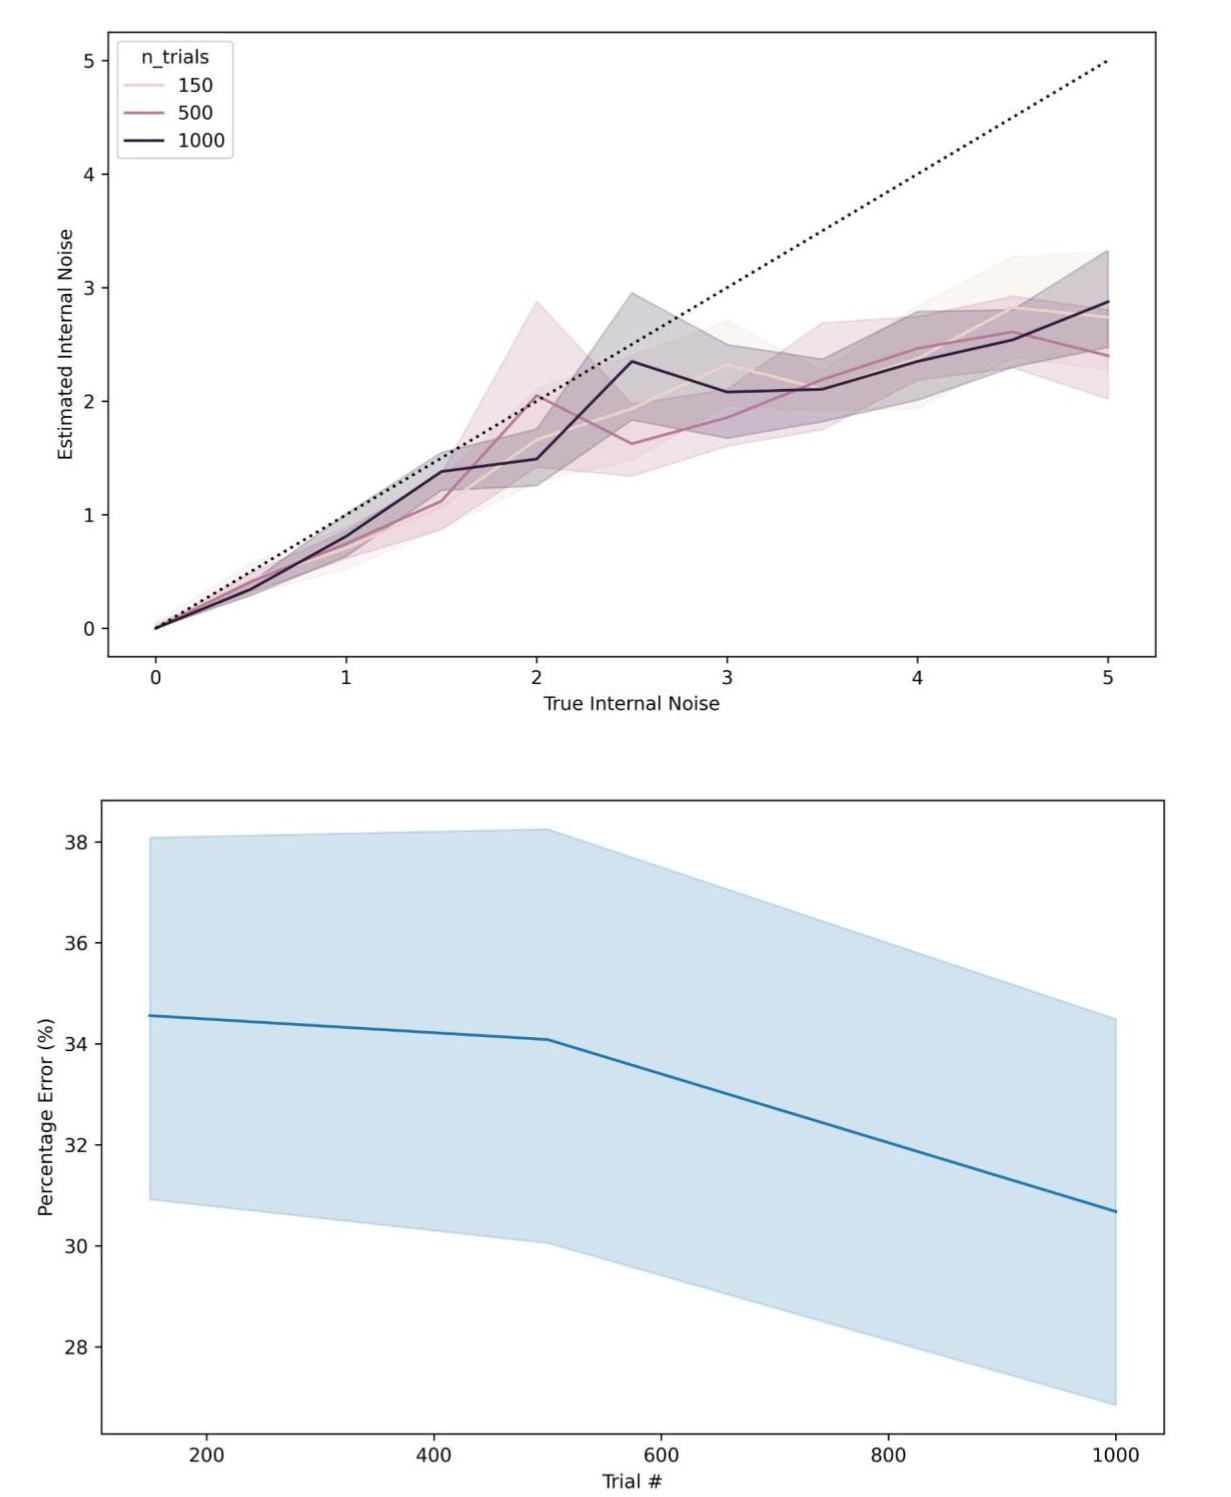
\includegraphics[width=14cm]{MainLayout/Images/internal_noise.jpg}
    \caption{Main Title for First Image \\ \small Subtitle for the first graphic.}
    \label{fig:internal_noise}
\end{figure}
 
\section{High-level processing}

\jj{faut-il présenter la revcor avec s+n vs n, puis dire que nous on ne fait pas ça; ou bien directement trouver une formulation b+n1 vs b+n2 qui correspond à ce qu'on fait en réalité ? }

In psychophysical experiments, noise is often added to all trials rather than separating them into distinct $signal+noise$ and $noise-only$ conditions. This approach reflects a deliberate effort to engage higher-level cognitive processes and to explore distributed, ecologically relevant features in a meaningful way.

Traditional signal+noise and noise-only paradigms are well-suited for studying low-level sensory processing, where individual features like luminance  (Barlow, 1956), orientation  (Jones, Anderson, \& Murphy, 2003), or frequency dominate on image stimuli \cite{dotsch_reverse_2012} or on auditory spectrogram\cite{varnet_how_2015}. However, many high-level cognitive tasks involve more complex, distributed features that cannot be easily isolated in such frameworks. For instance, facial expressions such as a smile rely on coordinated movements of facial muscles \cite{ponsot_uncovering_2018}, while auditory features like intonation or phoneme transitions are distributed across spectro-temporal patterns \cite{ponsot_cracking_2018}. These high-level features are not well-captured in low-level stimulus subspaces, where noise-only stimuli may lack meaningful structure.

By adding noise to all trials \cite{burred_cleese_2019}, researchers allow the natural complexity of stimuli to remain intact while introducing variability that can be regressed against participant responses. This approach enables a more efficient exploration of the stimulus space, isolating the subspace of features most relevant to participant judgments. For example, in reverse-correlation studies, applying noise to all trials facilitates the identification of high-level dimensions that influence responses, such as emotional expressions or vocal intonation.

\section {Discussion} 

In Chapter\ref{chap2}, we explored the biological basis of prosody perception, emphasizing its critical role in communication and social interaction after stroke. We also discussed the challenges posed by traditional assessment tools, which often fail to provide mechanistic and specific insights into deficits like aprosodia. These limitations highlight the need for approaches that move beyond descriptive measures to quantify prosody perception in a systematic and theory-driven way.

In Chapter\ref{chap3}, we took a step toward addressing these gaps by introducing possible mechanistic model rooted in computational psychophysics. Specifically, we examined psychophysical experiments such as reverse correlation to probe how participants process and represent prosodic cues. This framework allowed us to compute key variables:
\begin{itemize}
    \item Internal representations, estimated using classification images, to map the auditory features participants rely on for prosody judgments.
    \item Internal noise, quantified through double-pass experiments, to measure variability in the perceptual and decision-making processes.
\end{itemize}

These methods provide insights into what model may interpret prosody perception better by offering precise, computationally grounded metrics for understanding how individuals perceive and respond to prosodic stimuli.

Next chapter\ref{chap4} lays the groundwork for transitioning from theoretical exploration to empirical application. By combining the mechanistic models from Chapter 2 with real-world data, we aim to develop a framework that bridges theory, data, and computation. Computational psychophysics provides a powerful lens through which to study prosody perception, enabling us to:
\begin{itemize}
\item Apply models to actual data, testing their predictive power and robustness in quantifying deficits.
\item Explore individual differences in prosody perception, paving the way for personalized assessment tools.
\end{itemize}

This approach underscores the importance of a data-driven perspective that integrates computational rigor with experimental precision, facilitating the discovery of biomarkers for prosodic deficits like aprosodia and responding to the question that "Is Psychophysics Relevant for High-Level Processing?"